\documentclass{ExcelAtFIT}
%\documentclass[czech]{ExcelAtFIT} % when writing in CZECH
%\documentclass[slovak]{ExcelAtFIT} % when writing in SLOVAK

\usepackage{newtxmath}
\usepackage{amsmath}
\usepackage{amssymb}
\usepackage{graphicx}
\usepackage{enumitem}
\usepackage{multirow}
\usepackage{booktabs}
\usepackage{hhline}
\usepackage{arydshln}
\setlist{nolistsep}
\setlist{nosep}
\newcommand\scalemath[2]{\scalebox{#1}{\mbox{\ensuremath{\displaystyle #2}}}}

\def\uv#1{\iflanguage{british}{``#1''}{\quotedblbase #1\textquotedblleft}}

\usepackage[skip=0pt]{caption}

% \DeclareCaptionLabelSeparator{defffis}{ -- }
\captionsetup[table]{
    position=top,
    belowskip=0pt, % before caption
    aboveskip=0pt, % after caption
    justification=raggedright,
    format=plain, singlelinecheck=false,
} 
%--------------------------------------------------------
%--------------------------------------------------------
%	REVIEW vs. FINAL VERSION
%--------------------------------------------------------

%   LEAVE this line commented out for the REVIEW VERSIONS
%   UNCOMMENT this line to get the FINAL VERSION
%\ExcelFinalCopy


%--------------------------------------------------------
%--------------------------------------------------------
%	PDF CUSTOMIZATION
%--------------------------------------------------------

\hypersetup{
	pdftitle={Paper Title},
	pdfauthor={Author},
	pdfkeywords={Keyword1, Keyword2, Keyword3}
}

\lstset{ 
	backgroundcolor=\color{white},   % choose the background color; you must add \usepackage{color} or \usepackage{xcolor}; should come as last argument
	basicstyle=\footnotesize\tt,        % the size of the fonts that are used for the code
}

%--------------------------------------------------------
%--------------------------------------------------------
%	ARTICLE INFORMATION
%--------------------------------------------------------

\ExcelYear{2022}

\PaperTitle{Detection of pre-recorded messages in speech}

\Authors{Dominik Boboš*} 
\affiliation{*%
  \href{mailto:xbobos00@stud.fit.vutbr.cz}{xbobos00@stud.fit.vutbr.cz},
  \textit{Faculty of Information Technology, Brno University of Technology}}
%%%%--------------------------------------------------------
%%%% in case there are multiple authors, use the following fragment instead
%%%%--------------------------------------------------------
%\Authors{Jindřich Novák*, Janča Dvořáková**}
%\affiliation{*%
%  \href{mailto:xnovak00@stud.fit.vutbr.cz}{xnovak00@stud.fit.vutbr.cz},
%  \textit{Faculty of Information Technology, Brno University of Technology}}
%\affiliation{**%
%  \href{mailto:xdvora00@stud.fit.vutbr.cz}{xdvora00@stud.fit.vutbr.cz},
%  \textit{Faculty of Information Technology, Brno University of Technology}}

\Keywords{Detection of re-occurring sequences in audio --- Segmental dynamic time warping --- Recurrence quantification analysis --- Fuzzy string matching --- Bottleneck features --- Phoneme posteriors}

\Supplementary{\href{https://github.com/DominikBobos/VUT-FIT-Excel-Fit-2022}{Downloadable Code}}


%--------------------------------------------------------
%--------------------------------------------------------
%	ABSTRACT and TEASER
%--------------------------------------------------------


\Abstract{
Recognition of pre-recorded messages in speech such as "This number is not reachable" is useful for any follow-up speech data mining. 
To investigate the identification of redundant information in audio, it is necessary to have a large amount of data with the exact phrases repeated multiple times. Such a set is generated by mixing pre-recorded messages into phone calls with variations in speed, volume and repetitions. The created system tackles “known messages” and “unknown messages” scenarios by using approaches like clustering or detection in chunks. Dynamic time warping, approximate string matching and recurrent quantification analysis are compared, and finally, all mentioned techniques are combined to obtain a precise and efficient system.  
}

\Teaser{
	\TeaserImage{images/teaser.pdf}
}



%--------------------------------------------------------
%--------------------------------------------------------
%--------------------------------------------------------
%--------------------------------------------------------
\begin{document}

\startdocument


%--------------------------------------------------------
%--------------------------------------------------------
%	ARTICLE CONTENTS
%--------------------------------------------------------

%--------------------------------------------------------
%--------------------------------------------------------
%--------------------------------------------------------
%--------------------------------------------------------
\section{Introduction}
The typical scenario for investigating audio recordings starts with a large dataset. Storing a large amount of speech data comes with a lot of disadvantages. On one hand, the low-level problems like running out of free space. On the other hand, listening through unnecessary, repetitive data or time-consuming automatic processing.

Since these recordings are often telephone calls, many share typical features. For instance, ringing, voicemail message, music on hold or any pre-recorded message. The more recordings of telephone conversations, the higher the probability of occurrence of mentioned shared segments. These typically include pre-recorded operator messages (for instance, "Thank you for calling, please leave a message.", "Sorry the number you are calling does not answer at the moment, please try again later"). 

Detection could improve productivity for many professions, such as law enforcement agencies (LEA) or call centres. Hence the main objective is to minimise wasting time by listening to redundant information in speech data and decrease processing time by further automatic processing. That means that the requirement for the system is to have a fast and accurate solution with a minimum hardware load. Another requirement is to have a robust system working independently on the language, as with low-resource languages, it is not possible to use such techniques as automatic speech recognition. 

To find similar or identical parts effectively in a large dataset with nearly zero knowledge, it is essential to choose the methodology for tagging detected pre-recorded operator messages. Either mark an exact time in the phone call or provide a binary decision only -- whether the given recording contains pre-recorded speech.    

This paper presents two main scenarios how to achieve this task:
\label{intro}
\begin{enumerate}
    \item \textbf{Known messages scenario} -- This scenario is used to create \textit{reference clusters}. The cluster analysis is accomplished by provided labelled pre-recorded messages. Recordings are compared to reference clusters. 

\label{knownmessages}
    \item \textbf{Unknown messages scenario} -- Here the system does not know the pre-recorded messages and has to infer them as repeated parts of calls. This approach can be divided into the following tasks:
\label{unknownmessages}
    \begin{enumerate}[a)]
        \item Detection based on \textit{a recording itself} -- The process does not require any additional information, and the pre-recorded message is detected in itself. 

        \item Detection based on \textit{all files} -- Recordings are compared to all recordings in the set or by a chunk of the set. The new chunk is randomly chosen with every recording. 
    
        \item Detection based on \textit{clusters} -- Recordings are compared to the created clusters. The cluster analysis requires list of candidates. 
    \end{enumerate}
\end{enumerate}


This paper combines several techniques for searching repeating sequences in speech. From the basic ones like Dynamic Time Warping (DTW) -- to search the distance between two recordings, to more advanced ones like Recurrence Quantification Analysis (RQA) -- which analyses diagonal line segments in recurrence matrix. Approximate string matching (also known as Fuzzy string matching) is used to analyse the similarity between two phoneme strings. The best accuracy while preserving low processing time is achieved by the combination of all mentioned techniques.


\section{Used techniques}
\subsection{Dynamic Time Warping}
Even though the same person says the same sentence twice, it will never sound exactly the same. It may vary in length, speed, intonation, volume, pitch etc. Linear frame-by-frame matching of two sequences will fail, even though it is the same sentence. \textit{Dynamic time warping} (\textbf{DTW}) is an algorithm used to find the shortest distance and compare two time series when the time indices are not synchronised, the standard procedure is explained in \cite{MFCCDTW}. The comparison between linear matching and DTW distance matching is shown in Figure \ref{fig:EuclidDTW}. 

\begin{figure}[hbt]
	\centering
	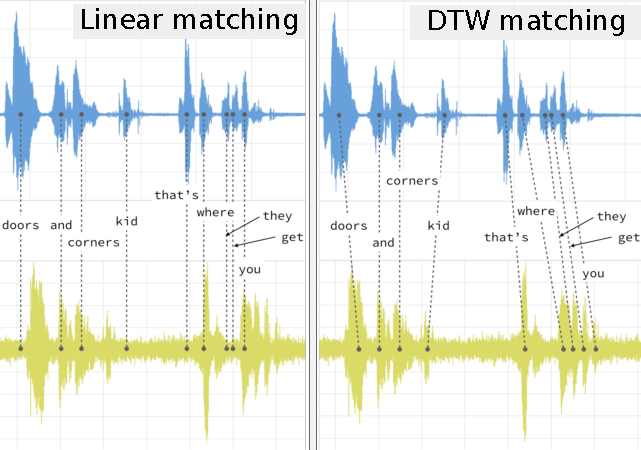
\includegraphics[width=\linewidth]{images/EuclideanDTWedited2.pdf}
	\caption{Comparison between linear matching and DTW matching on two speech recordings. \cite{DTWnotebook}.}
    \label{fig:EuclidDTW}
\end{figure}

\subsection{Segmental DTW}
DTW is finding one global optimal alignment path between the whole two sequences. This may be an issue for detecting similarities in sub-sequences. In Aren Jansen's work, \textit{Segmental Dynamic Time Warping} (\textbf{S-DTW}) is presented as a solution \cite{ArenJansen}. 
The principle of the S-DTW algorithm is to use other diagonals of an optimal alignment path for searching than the main diagonal. It consists of two main components: \texttt{i)} \textit{Global constraints}, which are restricting space a warping path can take while producing multiple alignment paths by changing starting and ending points in the same two input sequences, and \texttt{ii)} \textit{path trimming procedure} which excludes largely distorted regions of an alignment path by \textit{length-constrained minimum average} \emph{LCMA} \cite{SDTWpark2006unsupervised}.
A comparison between DTW and S-DTW for two utterances is shown in Figure \ref{fig:SDTWresult}.


\begin{figure}[hbt]
	\centering
	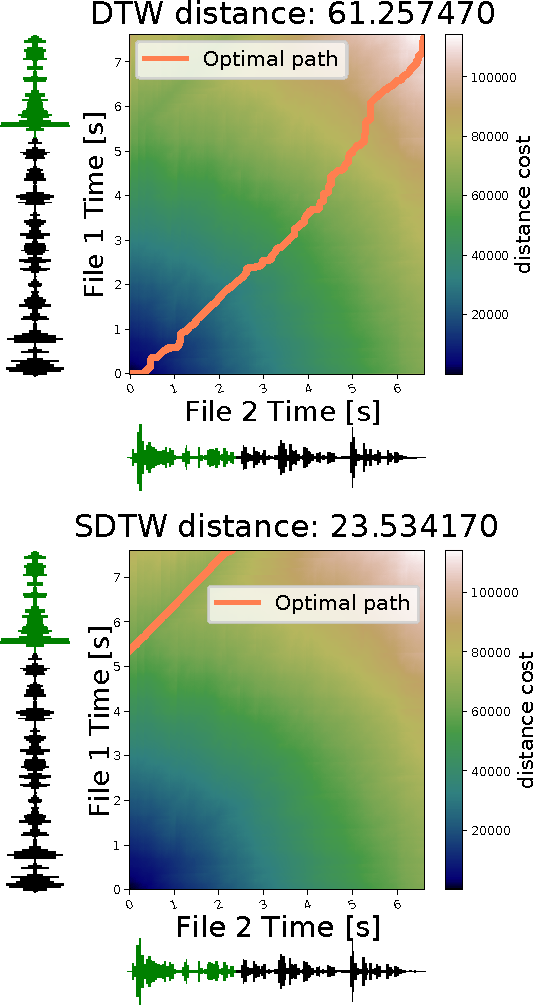
\includegraphics[width=0.8\linewidth]{images/DTW_SDTW_comparision2edited.pdf}
	\caption{DTW and S-DTW alignment paths of the two utterances, where File 1 contains the phrase "Brno University of Technology" at the beginning, while File 2 at the end.}
    \label{fig:SDTWresult}
\end{figure}


\subsection{Recurrence quantification analysis}
\textit{Recurrence quantification analysis} (\textbf{RQA}) is a method of nonlinear data analysis. RQA calculates the value of path alignments by dynamic programming \cite{LibrosaRQAref}. RQA provides objective quantification of important aspects revealed by the plot -- recurrence matrix (RM). Points in an RM that form diagonal line segments are considered to be deterministic (apart from the isolated points) \cite{RQAbook}.
The method is similar to DTW. However, instead of finding the shortest alignment path, in the RQA analysis, the longest alignment paths are selected. 
RQA quantifies the structure of RM by several metrics which are used as a weights \cite{RQAindices}. 
The used recipe for RQA is described in \cite{LibrosaRQAref}.

\subsection{Fuzzy string matching}
There are many use cases when it is desirable to know how similar one string is to another, such as text retrieval, signal processing, and computational biology. \textit{Fuzzy string matching} (\textbf{FSM}) (also known as Approximate string matching) is an algorithm for comparing two strings approximately. For instance, "I~ate a fresh green apple." is similar to "He eats fresh green apples." at the first sight, but not for the computer. 

\subsubsection*{Levenshtein distance}
\label{LevenshteinDistance}
The decent solution for quantifying the similarity is the \textit{Levenshtein Distance} (LD) (also known as \textit{"edit distance"}). It compares strings by several edit operations, such as deletion, insertion, and substitution of individual symbols. LD can be defined as the minimum cost of converting one string into another by using a sequence of edit operations \cite{LevenshteinDist}.


\section{Simulated dataset}
No publicly known solution exists for the problem, that means no dataset as well.   

To create a simulated dataset, the telephone operator pre-recorded messages were collected first: a total of \textbf{26 unique recordings} either downloaded from the internet or recorded from real telephone conversations. The messages are in English, Czech and Slovak. They were split into three categories: \texttt{A)} messages to occur at the beginning of the call, \texttt{B)} messages to occur anywhere through the call and \texttt{C)} messages to occur both at the beginning and the end of the call. All pre-recorded messages were pre-processed (removal of the initial silence and volume normalisation).

The next step is to mix the telephone operator messages with \textbf{517.13} hours of phone calls from the Switchboard corpus\footnote{\href{https://catalog.ldc.upenn.edu/LDC97S62}{LDC Switchboard-1 Release 2:\\ https://catalog.ldc.upenn.edu/LDC97S62}} in total of 4870 conversations. The conversations were trimmed to shorten calls to uniform (in terms of hours) eight categories from a 15-second-long to 180-second-long calls. For the mixing process, approximately 10\% of the trimmed phone calls were chosen -- 4260 calls. Also, 200 recordings of zero length calls were chosen -- the total number of calls is then \textbf{4460}. 

To get close to realistic data, each pre-recorded message is mixed into calls with varying speed (between 0.9 -- 1.1), volume gain (between -6dB -- +6dB) and varied repetition (between 0.8 to 30.0). The average length of a mixed pre-recorded message is around one minute.
The total count of the mixed pre-recorded messages is \textbf{4460} files of a total length of \textbf{150.66 hours}. The metadata of the changes made to the messages are preserved in the filename. 

The audio files are in 16-bit wave format with a standard sample rate of \textbf{8000 Hz}.
The prepared recordings were split into training and evaluation sets and their subsets used for development -- total numbers are presented in table \ref{tab:Database}. Each of the sets contains representatives of every pre-recorded telephone operator message -- just in a different ratio. With intention of creating a universal dataset for varied techniques of machine learning, "Train" and "Sub train" sets are created but not used in evaluations \cite{bobos}.

\begin{table}[hbt]
\centering
\caption{Total lengths in hours and counts of audio files in individual sets.}
\label{tab:Database}
\resizebox{\linewidth}{!}{%
\begin{tabular}{l|cccr} 
\toprule
\multicolumn{1}{c}{\begin{tabular}[c]{@{}c@{}}\\\\\textbf{Database}\end{tabular}} & \begin{tabular}[c]{@{}c@{}}\textbf{Raw }\\\textbf{ phone calls }\\\textbf{ [hours]}\end{tabular} & \begin{tabular}[c]{@{}c@{}}\textbf{Mixed calls }\\\textbf{ with messages }\\\textbf{ [hours]}\end{tabular} & \begin{tabular}[c]{@{}c@{}}\textbf{Total }\\\textbf{ [hours]}\end{tabular} & \multicolumn{1}{c}{\begin{tabular}[c]{@{}c@{}}\textbf{Total }\\\textbf{ (raw + mixed)}\\\textbf{ [count]}\end{tabular}}  \\ 
\hline
\textbf{Train}                                                                    & 339.31                                                                                           & 117.63                                                                                                     & \textbf{456.94}                                                            & \textbf{35953}                                                                                                           \\ 
\hline
\textbf{Eval}                                                                     & 126.62                                                                                           & 37.10                                                                                                      & \textbf{163.72}                                                            & \textbf{11467}                                                                                                           \\ 
\hline
\textbf{Sub train}                                                                & 16.83                                                                                            & 30.62                                                                                                      & \textbf{47.45}                                                             & \textbf{1394}                                                                                                            \\ 
\hline
\textbf{Sub eval}                                                                 & 4.31                                                                                             & 6.48                                                                                                       & \textbf{10.79}                                                             & \textbf{374}                                                                                                             \\
\bottomrule
\end{tabular}
}

\end{table}



\section{Baselines}
This section provides details about the baseline systems used for detecting the pre-recorded messages. Their input can be \texttt{i)} either the recording itself (used in RQA approach) and \texttt{ii)} pre-recorded messages detection on all files or chunks of the set (used in DTW and FSM approaches).
The results provide binary decision only – either the audio contains the message or not.

For the work, I used standard MFCC features\footnote{\href{https://python-speech-features.readthedocs.io/en/latest/}{Python package python\_speech\_features: https://python-speech-features.readthedocs.io/en/latest/}}, phoneme posteriors\footnote{\href{https://speech.fit.vutbr.cz/software/phoneme-recognizer-based-long-temporal-context}{Phoneme recogniser based on long temporal context \cite{SchwarzPhonerec}: https://speech.fit.vutbr.cz/software/phoneme-recognizer-based-long-temporal-context}} and bottleneck features\footnote{\href{https://speech.fit.vutbr.cz/software/but-phonexia-bottleneck-feature-extractor}{BUT/Phonexia Bottleneck feature extractor \cite{BottleneckExtractor}: https://speech.fit.vutbr.cz/software/but-phonexia-bottleneck-feature-extractor}}.

\textit{Detection error trade-off} (DET) curves \cite{DETcurve} and \textit{Equal error rate} (EER) \cite{EER} are used for evaluation.
For measuring the quality of clustering, metrics like purity, rand index, normalised mutual information are used, more in book \cite{ClusterEvalBook}. 


\subsection{DTW approach}
\label{DTWapproach}
DTW gives optimal results when comparing similarly long time series with isolated words. However, in our case, the recordings are of various lengths. Also, the similar parts are repeated unevenly, and the position of a pre-recorded message could be anywhere in the file. The first important step is to find candidates of similar parts between two recordings on the DTW alignment path and then find DTW distance between the candidates. 
\subsubsection*{Searching for candidates}
To find the candidates for determining similarity, the DTW warping path is computed first and then analysed. The algorithm finds the similarities by looking back to the previous steps the warping path has taken. In a DTW warping path, 3 moves are possible: i) \textit{diagonal}, ii) \textit{horizontal} and iii) \textit{vertical}. 
Three types of moves that a two-step pair can get:  
\begin{itemize}
    \item The \textit{"good trend"} (GT) type happens when the current step is in diagonal direction. The direction of the previous step does not matter in this case.
    \item The \textit{"false trend"} (FT) type happens when the two-step pair consists of two horizontal moves or two vertical moves.
    \item The \textit{"neutral trend"} (NT) type happens when the two-step pair consists of one vertical and one horizontal moves or one is in the diagonal direction.
\end{itemize}

The idea of the experimental function for finding candidates is to start detecting the similarity when the diagonal move occurs. Then each step is evaluated and the corresponding point is added to the list.

FT type increments the false-trend variable and the constant false trend variable. GT type increments the good-trend variable and resets the variable responsible for monitoring the constant false-trend types. NT type resets only the constant false-trend variable. 

The detection ends when the constant false trend is larger than the given threshold $\sigma$. Then the quality of the detected part of a sequence is evaluated. First, the length of the list needs to be longer than $\delta$ frames, which means $\delta/100$ seconds. Sequences longer than $\delta$ are scored by the ratio of the triangle created by the warping path, y-axis and x-axis. If the ratio falls in given interval $\tau$, the detected line is a good candidate. The whole process repeats until the end of the warping path. In the presented baseline system, the variables are set accordingly: $\sigma = 25$, $\delta = 200$, and $\tau \in \langle0.9, 1.1\rangle$. The behaviour and the results of the algorithm is shown in Figure \ref{fig:BaseDTW}.

\begin{figure}[hbt]
	\centering
	\tmpframe{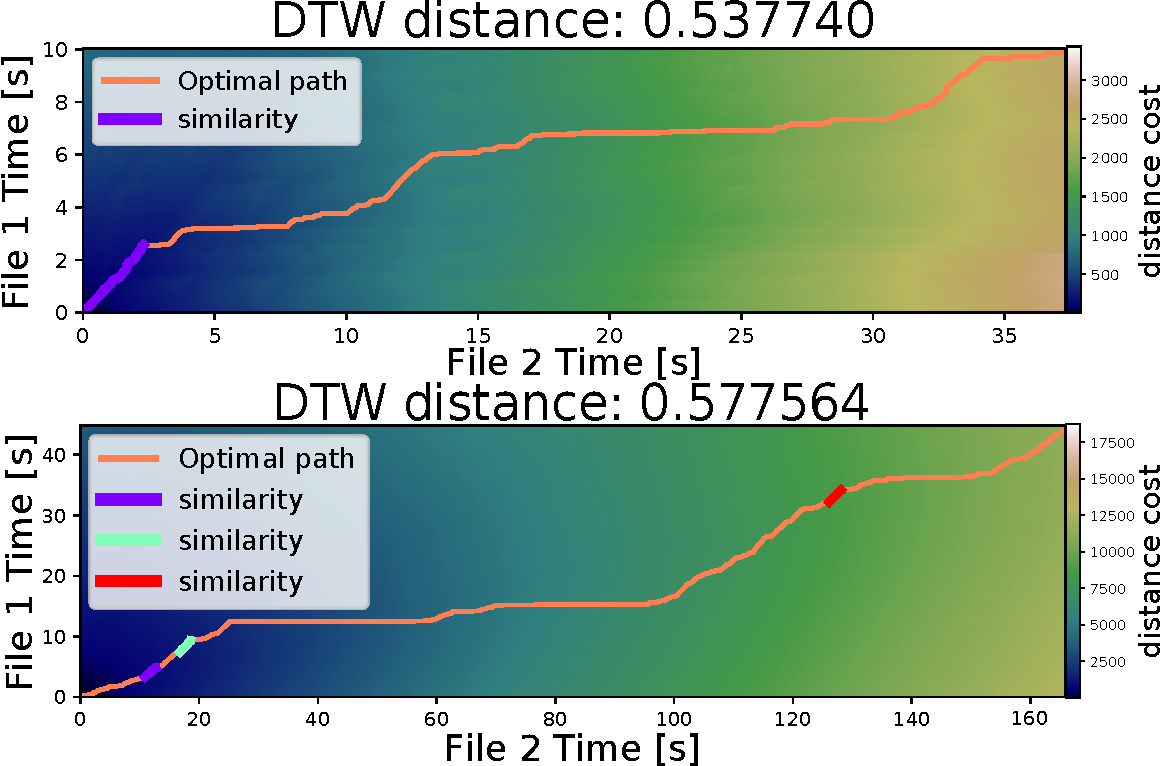
\includegraphics[width=\linewidth]{images/baseDTWbothedited.pdf}}
	\caption{DTW path with applied candidates detection algorithm. The top one with one candidate is later classified as a hit. The bottom alignment obtains several candidates, but none of them resulted in a hit.}
    \label{fig:BaseDTW}
\end{figure}


The proposed solution for the baseline DTW system is to compare every feature vector and its found candidates with all others. By using a brute-force approach, it is immediately an $O(n^2)$ problem. However, a little trick is performed to get a better constant. Each file is compared to a randomly chosen chunk of all recordings. The chunk size is $1/8$ of the set. As the idea of detecting the pre-recorded messages is to find parts repeated several times, at least one should appear in the reduced bunch. Performance of DTW system does not meet the required accuracy and fast processing time as shown in table \ref{tab:BaseDTW}.


\begin{table}[hbt!]
\centering
\caption{Results of the baseline DTW system on "Sub eval" dataset.}
\label{tab:BaseDTW}
\resizebox{0.7\linewidth}{!}{%
\begin{tabular}{l|ccc} 
\hline
\multicolumn{1}{l}{\begin{tabular}[c]{@{}l@{}}\\\\\\\textbf{Features}\end{tabular}} & \begin{tabular}[c]{@{}c@{}}\textbf{Average}\\\textbf{time}\\\textbf{ of one file}\\\textbf{ [seconds]}\end{tabular} & \begin{tabular}[c]{@{}c@{}}\textbf{CPU-core}\\\textbf{time}\\\textbf{ [hours]}\end{tabular} & \textbf{EER}      \\ 
\hline
\textbf{MFCC}                                                                       & 244.39                                                                                                              & 8.46                                                                                        & \textbf{41.17\%}  \\ 
\hline
\begin{tabular}[c]{@{}l@{}}\textbf{Phoneme}\\\textbf{posteriors}\end{tabular}       & 284.30                                                                                                              & 9.79                                                                                        & \textbf{30.48\%}  \\ 
\hline
\textbf{Bottleneck}                                                                 & 477.49                                                                                                              & 16.53                                                                                       & \textbf{29.41\%}  \\
\hline
\end{tabular}
}
\end{table}
\subsection{RQA approach}
The RQA approach is based on Aren Jansen's work \cite{ArenJansen}. RQA analysis expects the similarity matrix at the input -- a~cosine distance is used for creating the matrix. The self-similarity diagonal is removed. Default settings for RQA from Librosa package \footnote{\href{https://zenodo.org/badge/6309729.svg}{Librosa 0.8.0 on Zenodo:\\https://zenodo.org/badge/6309729.svg}} are used, together with \textit{affinity mode} and \textit{knight moves} on.

As the telephone operator messages are often repeated several times within the recording, the recurrence matrix is computed for one file at a time only. This approach allows working in linear time-space of $O(n)$ as each file is analysed only once. Samples shorter than 3 seconds are not included, as short speech conversation should not be present in the analysis for correct computation. Shorter recordings are evaluated with a high penalty score. 

Next, the heuristic to filter out false alarms from RQA analysis is to accept the best alignment sequence longer than $\delta$ only. Such a heuristic, of $\delta = 2.5$ seconds, helps to reduce false alarms, as those alignment paths usually happen to be only a word or a short inactive part. An unsatisfactory result is evaluated with a large score. 

The alignment path from RQA analysis is scored by the sum of the similarity points of the longest similarity path, divided by the length of the path. Scores below the threshold $\phi$ are marked as a hit. Lower processing time is achieved by frame reduction (FR) optimisation (more in subsection \ref{optimisations}). MFCC features perform significantly the best over the phoneme posteriors and bottleneck features. The average processing time for one file and overall performance is presented in table \ref{tab:RQADETs}.

\begin{table}[hbt]
\centering
\caption{Processing time and evaluation result of RQA system with different settings. FR stands for frame reduction, M means MFCC features, PP -- phoneme posteriors, BN -- bottleneck features.}
\label{tab:RQADETs}
\resizebox{\linewidth}{!}{%
\begin{tabular}{c|ccc||ccc||ccc} 
\hline
\multicolumn{1}{c}{}                                      & \multicolumn{3}{c}{\begin{tabular}[c]{@{}c@{}}Average time\\ {[}seconds]\end{tabular}} & \multicolumn{3}{c}{\begin{tabular}[c]{@{}c@{}}Total time\\ {[}minutes]\end{tabular}} & \multicolumn{3}{c}{\begin{tabular}[c]{@{}c@{}}EER \\ {[}\%]\end{tabular}}  \\ 
\hline
Features                                                  & \multirow{2}{*}{M} & \multirow{2}{*}{PP} & \multirow{2}{*}{BN}                         & \multirow{2}{*}{M} & \multirow{2}{*}{PP} & \multirow{2}{*}{BN}                       & \multirow{2}{*}{M} & \multirow{2}{*}{PP} & \multirow{2}{*}{BN}             \\ 
\cline{1-1}
\multicolumn{1}{l|}{Dataset}                              &                    &                     &                                             &                    &                     &                                           &                    &                     &                                 \\ 
\hline
\begin{tabular}[c]{@{}c@{}}Sub eval \\ FR=5\end{tabular}  & 2.06               & 2.56                & 3.08                                        & 12.84              & 16.95               & 19.20                                     & \textbf{1.60}    & 15.50             & 16.04                         \\ 
\hline
\begin{tabular}[c]{@{}c@{}}Sub eval \\ FR=10\end{tabular} & 1.61               & 2.36                & 2.11                                        & 10.03              & 14.72               & 13.17                                     & 12.30            & 20.86             & 22.99                         \\ 
\hline
\begin{tabular}[c]{@{}c@{}}Sub eval \\ FR=20\end{tabular} & \textbf{1.05}      & 1.68                & 1.55                                        & \textbf{6.52}      & 10.45               & 9.65                                      & 32.62            & 28.88             & 27.81                         \\ 
\hhline{====::===::===}
\begin{tabular}[c]{@{}c@{}}Eval \\ FR=5\end{tabular}      & \textbf{1.92}      & 2.17                & 2.91                                        & \textbf{365.73}    & 412.84              & 544.65                                    & \textbf{1.34}    & 6.68              & 10.38                         \\
\hline
\end{tabular}
}
\end{table}

\subsection{FSM approach}
Fuzzy phoneme string matching approach is based on \textit{Levenshtein distance}.
First, the text file output from a phoneme recogniser by Petr Schwarz \cite{SchwarzPhonerec} is imported and parsed. The example of the phoneme recogniser output can be as following: 
\begin{verbatim}
  0 1300000 s -12.662029
  1300000 2700000 e -13.111244
  2700000 14900000 pau -118.012054
  14900000 15300000 n -3.924468
\end{verbatim}
The first two columns represent time interval of a phoneme, where 1 second is represented as $10000000$. The third column shows an occurred phoneme. The last one provides the duration of the occurred phoneme. This output is parsed into list of lists with following structure: \texttt{\[[\,[frames],\-[lengths],\-[index\_map],\-string\,]\]}, where \texttt{[frames]} represents the list of intervals (with trimmed 5 zeros from the end), \texttt{[lengths]} is the list of phoneme durations in hundredths of seconds, \texttt{[index\_max]} is the list of occurred phonemes at the corresponding index, \texttt{string} is the phoneme string of the whole recording with replaced "pau" labels to spaces, which is used in comparison.
The output from the example would be parsed into:
\begin{verbatim}
[ 
 [[0,13],[13,27],[27,149],[149,153]],
 [12.662, 13.111, 118.012, 3.924],
 ['s', 'e', 'pau', 'n'],
 "se n"
]
\end{verbatim}
Such a parsing allows to convert between features and to return just needed parts of a string.
A \textit{partial ratio} function from \textit{FuzzyWuzzy}\footnote{\href{https://pypi.org/project/fuzzywuzzy/}{FuzzyWuzzy 0.18.0 on PyPI:\\https://pypi.org/project/fuzzywuzzy/}} package tackles the problem with uneven phoneme string lengths. Let assume a pair of strings of the same pre-recorded message. One is repeated three times, the other one is repeated once. Basic ratio function returns score $60\%$, while partial ratio function returns $84\%$. However, this approach causes that even one word "you" compared to a whole sentence with "you" somewhere returns a score of $100\%$. This can be fixed by applying brute force – ignore $100\%$ scores, as it is almost certain that it is shown case. It is important to realise that even the same telephone operator messages will not probably return a score of 100\%. The algorithm is based on comparing each phoneme string to another -- same as the DTW approach. Accordingly, it is optimised by chunking. The size of randomly chosen chunks from the set is $1/4$ of all recordings. 

\begin{table}[hbt]
\centering
\caption{Performance of baseline fuzzy string matching system.}
\label{tab:FuzzyBaseResults}
\resizebox{0.8\linewidth}{!}{%
\begin{tabular}{l|c|c|c} 
\hline
\multicolumn{1}{l}{\begin{tabular}[c]{@{}l@{}}\\\textbf{Dataset}\end{tabular}} & \multicolumn{1}{c}{\begin{tabular}[c]{@{}c@{}}\textbf{Average time}\\\textbf{ [seconds]}\end{tabular}} & \multicolumn{1}{c}{\begin{tabular}[c]{@{}c@{}}\textbf{Total time}\\\textbf{ [hours]}\end{tabular}} & \begin{tabular}[c]{@{}c@{}}\textbf{EER}\\\textbf{ [\%]}\end{tabular}  \\ 
\hline
\textbf{Sub eval}                                                              & 29.57                                                                                                  & 3.07                                                                                               & \textbf{18.18\%}                                                      \\ 
\hline
\textbf{Eval}                                                                  & 37.14                                                                                                  & 102.53                                                                                             & \textbf{33.14\%}                                                      \\
\hline
\end{tabular}
}
\end{table}

\section{Experiments}
This section describes experiments and results to proposed baselines, clustering techniques and optimisations.
\subsection{Optimisations}
\label{optimisations}
Two main optimisations are used for decreasing processing time: \texttt{i)} caching and \texttt{ii)} frame averaging.

\textit{Caching} is the process of storing copies of files in a temporary storage. A~cache is a dictionary -- the key is the file name, and the value is the list with all components needed for the present system for further processing. This simple improvement rapidly reduce processing time by almost 80\% in some cases. 

\textit{Frame averaging} (or reduction) is a process of reducing the size of the feature vector.
Two proposed methods for frame averaging is presented: \texttt{i)} dimensions reduction and \texttt{ii)} reduction in a time axis.

\textit{Dimensions reduction} -- The posteriors feature vector represents three states for each one phoneme, making it 138 elements long. To reduce computation time, posteriors of triplets of states are summed to create posterior of one phoneme class.


\textit{Reduction in a time axis} -- Each second in an array is represented by hundred frames. The idea is to get a mean value of $n$ frames to minimise computation time while preserving as much information as possible. Used in RQA approach and S-DTW clustering.
        
    
\subsection{Clustering}
\label{Clustering}
Two types of clusters are used in evaluation: \texttt{i)} reference cluster -- created by labelled pre-recorded messages (known-messages scenario) and \texttt{ii)} predicted cluster -- created by list of candidates from RQA analysis (unknown-messages scenario).

Clustering is performed to improve accuracy and decrease processing time. Clustering removes the necessity to compare to every candidate and compare to representatives of cluster classes only.

The clustering process consists of two steps. First step -- Voice Activity Detection (VAD) and filtering\footnote{\href{https://github.com/wiseman/py-webrtcvad}{Used VAD for filtering -- py-webrtcvad on GitHub (used under MIT license): https://github.com/wiseman/py-webrtcvad}}. RQA analysis is performed and only non-empty list of frames from the analysis are preserved. Next, VAD is applied to the output from the analysis.

Second step -- dividing candidates into classes by using S-DTW\footnote{\href{https://github.com/gray0302/seg-dtw}{S-DTW implementation based on \cite{SDTWpark2006unsupervised} by gray0302 on GitHub. The implementation is modified to suit the needs: https://github.com/gray0302/seg-dtw}}. S-DTW clustering is performed on the filtered RQA analysis from step one. The clustering is based on Agglomerative Hierarchical Clustering (AHC). Every cluster is sorted by the lengths of the element --  the shortest recordings are at the top.

The process of creating reference (ground-truth) clusters for evaluation and experiments is based on known messages and their labels. The filename provides information about the message ID, the start and end of the message. Every message ID represents one class -- one cluster (of the total of 25 clusters). Every cluster is sorted the same as the automatic one.
The performance of the clustering is shown in tables \ref{tab:ClusteringEvaluation}, \ref{tab:ClusteringEvaluationTime}. MFCC provides the best processing time, however bottleneck features shows decent accuracy even with high frame reduction. The best speed-accuracy trade-off is with the $FR=20$.

\begin{table}[hbt]
\centering
\caption{Clustering performance evaluation by several metrics on different features like MFCC features (M), phoneme posteriors (PP), and bottleneck features (BN) with various settings of frame reduction (FR).}
\label{tab:ClusteringEvaluation}
\resizebox{\linewidth}{!}{%
\begin{tabular}{l|c|c|c||c|c|c||c|c|c} 
\hline
\multicolumn{1}{l}{\begin{tabular}[c]{@{}l@{}}\\\textbf{Metric}\end{tabular}} & \multicolumn{3}{c}{\textbf{Purity}}                                                & \multicolumn{3}{c}{\textbf{Rand Index}}                                            & \multicolumn{3}{c}{\textbf{NMI}}                                                    \\ 
\hline
\textbf{Features}                                                             & \multicolumn{1}{c}{\textbf{M}} & \multicolumn{1}{c}{\textbf{PP}} & \textbf{BN}     & \multicolumn{1}{c}{\textbf{M}} & \multicolumn{1}{c}{\textbf{PP}} & \textbf{BN}     & \multicolumn{1}{c}{\textbf{M}} & \multicolumn{1}{c}{\textbf{PP}} & \textbf{BN}      \\ 
\hline
\begin{tabular}[c]{@{}l@{}}\textbf{Sub eval}\\\textbf{FR = 10}\end{tabular}   & \textbf{0.88 }                & 0.87                           & 0.82           & \textbf{0.99 }                & 0.98                           & 0.98           & \textbf{0.93 }                & 0.92                           & 0.92            \\ 
\hline
\begin{tabular}[c]{@{}l@{}}\textbf{Sub eval}\\\textbf{FR = 20}\end{tabular}   & 0.66                          & 0.68                           & 0.81           & 0.93                          & 0.96                           & 0.98           & 0.82                          & 0.80                           & 0.92            \\ 
\hline
\begin{tabular}[c]{@{}l@{}}\textbf{Sub eval}\\\textbf{FR = 30}\end{tabular}   & 0.43                          & 0.43                           & 0.80           & 0.90                          & 0.86                           & 0.98           & 0.68                          & 0.56                           & 0.92            \\ 
\hline
\begin{tabular}[c]{@{}l@{}}\textbf{Sub eval}\\\textbf{FR = 40}\end{tabular}   & 0.31                          & 0.33                           & 0.77           & 0.83                          & 0.75                           & 0.97           & 0.54                          & 0.45                           & 0.90            \\ 
\hhline{====::===::===}
\begin{tabular}[c]{@{}l@{}}\textbf{Eval}\\\textbf{FR = 20}\end{tabular}       & 0.55                          & 0.66                           & \textbf{0.77 } & 0.88                          & 0.95                           & \textbf{0.97 } & 0.74                          & 0.75                           & \textbf{0.87 }  \\
\hline
\end{tabular}
}
\end{table}


\begin{table}[hbt]
\centering
\caption{Processing time of RQA system.}
\label{tab:ClusteringEvaluationTime}
\resizebox{0.5\linewidth}{!}{%
\begin{tabular}{l|c|c|c} 
\hline
\multicolumn{4}{c}{\begin{tabular}[c]{@{}c@{}}\textbf{Total Time}\\\textbf{ [minutes]}\end{tabular}}                                                          \\ 
\hline
\textbf{Features}                                                           & \multicolumn{1}{c}{\textbf{M}} & \multicolumn{1}{c}{\textbf{PP}} & \textbf{BN}  \\ 
\hline
\begin{tabular}[c]{@{}l@{}}\textbf{Sub eval}\\\textbf{FR = 10}\end{tabular} & \textbf{18.30 }                & 141.04                          & 288.90       \\ 
\hline
\begin{tabular}[c]{@{}l@{}}\textbf{Sub eval}\\\textbf{FR = 20}\end{tabular} & 4.93                           & 28.51                           & 58.20        \\ 
\hline
\begin{tabular}[c]{@{}l@{}}\textbf{Sub eval}\\\textbf{FR = 30}\end{tabular} & 2.20                           & 8.67                            & 17.93        \\ 
\hline
\begin{tabular}[c]{@{}l@{}}\textbf{Sub eval}\\\textbf{FR = 40}\end{tabular} & 1.76                           & 6.52                            & 11.15        \\ 
\hline\hline
\begin{tabular}[c]{@{}l@{}}\textbf{Eval}\\\textbf{FR = 20}\end{tabular}     & \textbf{183.57 }               & 237.97                          & 217.63       \\
\hline
\end{tabular}
}
\end{table}

\subsection{Combination of all techniques}
The final system combines all created systems to get the best performance. This experiment uses both reference clusters and clusters created by a list of candidates from RQA analysis and S-DTW AHC clustering.
This experiment is performed by \texttt{i)} clustering and \texttt{ii)} FSM evaluation afterwards.  

\textit{Clustering} -- the same process as described in subsection \ref{Clustering}, where frame reduction of $FR=20$ is used. Used S-DTW clusters are created from the "Eval" dataset from all available features. 

\textit{FSM evaluation} -- each testing file is compared to the first three elements of each cluster class. Used FSM in the experiment is modified to apply so called \textit{pause analysis}. In pause analysis, all silent parts longer than 2 seconds are declared as dividing points. Then the lengths of the segmented lists are checked. If the segment is shorter than 50 elements of the list, the segmented part is removed from the candidates. The pause-analysis modification of the baseline fuzzy string matching system aims to solve the main issue with the baseline system by segmenting the recordings. Results of the final system is shown in Figure \ref{fig:ClusterFuzzyDET} and table \ref{tab:ClusterFuzzy}. 


\begin{figure}[hbt]
	\centering
	\tmpframe{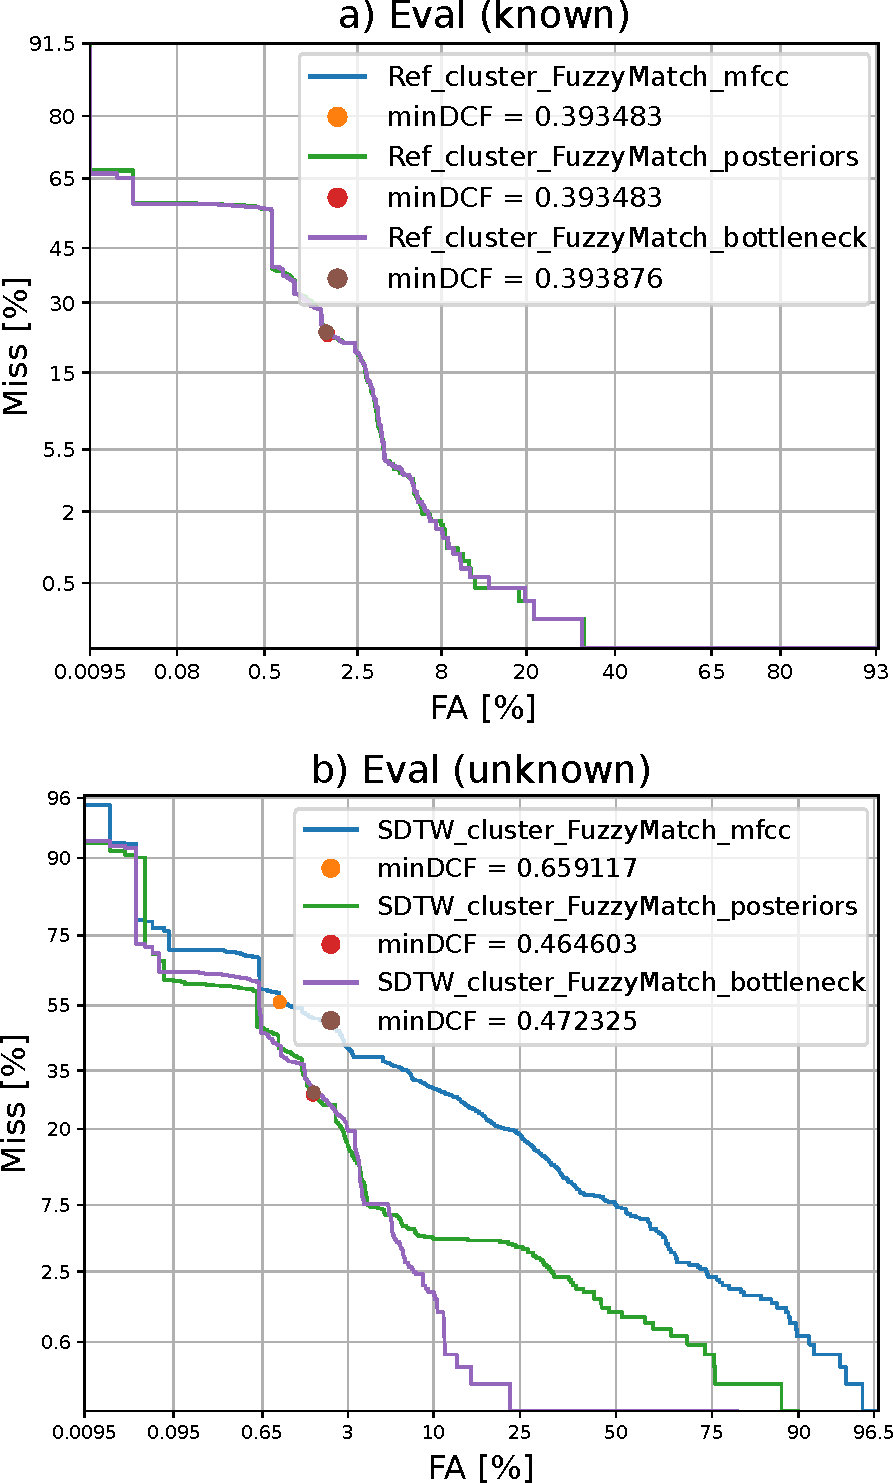
\includegraphics[width=0.95\linewidth]{images/AllBIGRQAclusters_Fuzzyedited.pdf}}
	\caption{Performance of the S-DTW cluster + fuzzy string matching system on the "Eval" dataset. The system works with both known messages a) and unknown messages b).}
    \label{fig:ClusterFuzzyDET}
\end{figure}


\begin{table}[hbt]
\centering
\caption{Results of final system. The system works with both known messages (reference cluster) and unknown messages (S-DTW cluster).}
\label{tab:ClusterFuzzy}
\resizebox{\linewidth}{!}{%
\begin{tabular}{l|ccc|ccc|ccc} 
\hline
\multicolumn{1}{l}{\begin{tabular}[c]{@{}l@{}}\\\textbf{Ref~}\\\textbf{cluster}\end{tabular}}                                       & \multicolumn{3}{c}{\begin{tabular}[c]{@{}c@{}}\textbf{Average time}\\\textbf{[seconds]}\end{tabular}}                   & \multicolumn{3}{c}{\begin{tabular}[c]{@{}c@{}}\textbf{Total time}\\\textbf{[hours]}\end{tabular}}                    & \multicolumn{3}{c}{\begin{tabular}[c]{@{}c@{}}\textbf{EER}\\\textbf{[\%]}\end{tabular}}                                               \\ 
\hline
\textbf{Features}                                                                                                                   & \textbf{M}          & \textbf{PP}          & \textbf{BN}                                                                & \textbf{M}          & \textbf{PP}          & \textbf{BN}                                                             & \textbf{M} & \textbf{PP}                                                                  & \textbf{BN}                               \\ 
\hline
\textbf{Sub eval}                                                                                                                   & 6.68                & 5.98                 & \textbf{5.96 }                                                             & 0.69                & 0.62                 & \textbf{0.62 }                                                          & 1.60       & 1.60                                                                         & \textbf{1.60}                             \\ 
\hline\hline
\textbf{Eval}                                                                                                                       & 17.35               & \textbf{12.06 }      & 19.78                                                                      & 9.12                & \textbf{6.30 }       & 10.15                                                                   & 4.28       & \textbf{4.28}                                                                & 4.30                                      \\ 
\hdashline
\multicolumn{1}{l}{\begin{tabular}[c]{@{}l@{}}\textbf{\textbf{}}\\\textbf{\textbf{S-DTW~}}\\\textbf{\textbf{cluster}}\end{tabular}} & \multicolumn{3}{c}{\begin{tabular}[c]{@{}c@{}}\textbf{\textbf{Average time}}\\\textbf{\textbf{[seconds]}}\end{tabular}} & \multicolumn{3}{c}{\begin{tabular}[c]{@{}c@{}}\textbf{\textbf{Total time~}}\\\textbf{\textbf{[hours]}}\end{tabular}} & \multicolumn{3}{c}{\begin{tabular}[c]{@{}c@{}}\textbf{EER}\\\textbf{[\%]}\end{tabular}}                                               \\ 
\hline
\textbf{\textbf{Features}}                                                                                                          & \textbf{\textbf{M}} & \textbf{\textbf{PP}} & \textbf{\textbf{BN}}                                                       & \textbf{\textbf{M}} & \textbf{\textbf{PP}} & \textbf{\textbf{BN}}                                                    & \textbf{M} & \textbf{PP}                                                                  & \textbf{BN}                               \\ 
\hline
\textbf{Sub eval}                                                                                                                   & \textbf{0.79}       & 3.91                 & 3.73                                                                       & \textbf{0.08}       & 0.41                 & 0.39                                                                    & 13.90      & \textbf{\textbf{\textbf{\textbf{\textbf{\textbf{\textbf{\textbf{2.14}}}}}}}} & 6.41                                      \\ 
\hline\hline
\textbf{Eval}                                                                                                                       & 1.57                & 1.57                 & \textbf{1.43}                                                              & 4.99                & 6.39                 & \textbf{4.54}                                                           & 20.48      & 6.34                                                                         & \textbf{\textbf{\textbf{\textbf{5.77}}}}  \\
\hline
\end{tabular}
}
\end{table}

\section{Conclusion and Future Work}
In this paper, methods for detecting repetitive parts across audio recording sets were presented. The research aimed especially at searching for pre-recorded telephone operator messages in speech conversations.

This paper took a deeper look at three techniques: Dynamic time warping, recurrence quantification analysis and fuzzy phoneme string matching. The main idea was to focus on the techniques when the system runs without the knowledge of the messages. The main goal was to find the most accurate and fastest approach.

To decide which system is the best, it was necessary to simulate a dataset. It was accomplished by mixing the operator messages into the Switchboard corpus while changing the speed, volume gain and a number of repetitions.

RQA performs the best among the three baseline methods. The bottleneck features bring the highest accuracy and MFCC features the fastest processing time. To decrease computation time, caching and frame averaging was applied. 
In the experiments, the best performance is achieved by all techniques combined. 

For future research, voice biometrics techniques for creating voice-prints of a speaker is the point of interest and how to integrate the method into the presented workflow. 

\section*{Acknowledgements}
I would like to thank my supervisor prof. Dr. Ing. Jan Černocký for valuable suggestions and friendly approach.

%--------------------------------------------------------
%--------------------------------------------------------
%--------------------------------------------------------
%	REFERENCE LIST
%--------------------------------------------------------
%--------------------------------------------------------
\phantomsection
\bibliographystyle{unsrt}
% \bibliographystyle{enplain}
\bibliography{bibliography}

%--------------------------------------------------------
%--------------------------------------------------------
%--------------------------------------------------------
\end{document}